%%%%%%%%%%%%%%%%%%%%%%%%%%%%%%%%%%%%%%%%%%%%%%%%%%%%%%%%%%%%%%%%%%%%%%%%%%%%%%
%   Sample paper (in LaTeX2e) for Annales Univ. Sci. Budapest., Sect. Comp.  %
%                                                                            %
%                       http://ac.inf.elte.hu                                %
%                                                                            %
%%%%%%%%%%%%%%%%%%%%%%%%%%%%%%%%%%%%%%%%%%%%%%%%%%%%%%%%%%%%%%%%%%%%%%%%%%%%%%




%%%%%%%%%%%%%%%%%%%%%%%%%%%%%%%%%%%%%%%%%%%%%%%%%%%%%%%%%%%%%%%%%%%%%%%%%%%%%%
%%%%%%%%%%%%%%%%%%%%%%%%%%%%%%%%%%%%%%%%%%%%%%%%%%%%%%%%%%%%%%%%%%%%%%%%%%%%%%
%%                                                                          %%
%%                             IMPORTANT:                                   %%
%%                  In case of any problems contact                         %%
%%                        ac@compalg.inf.elte.hu                            %%
%%                                                                          %%
%%%%%%%%%%%%%%%%%%%%%%%%%%%%%%%%%%%%%%%%%%%%%%%%%%%%%%%%%%%%%%%%%%%%%%%%%%%%%%
%%%%%%%%%%%%%%%%%%%%%%%%%%%%%%%%%%%%%%%%%%%%%%%%%%%%%%%%%%%%%%%%%%%%%%%%%%%%%%


\documentclass[10pt,leqno,twoside]{article}
\usepackage{graphicx}
\usepackage{annal-latex}
\usepackage{makeidx,latexsym,amssymb}
%%%%%%%%%%%%%%%%%%%%%%%%%%%%%%%%%%%%%%%%%%%%%%%%%%%%%%%%%%%%%%%%%%%%%%%%%%%%%%%%%%%%%%%%%%%%%%%
%%%% Your numbering system for theorems etc. may be different from the one suggested below. %%%
%%%%%%%%%%%%%%%%%%%%%%%%%%%%%%%%%%%%%%%%%%%%%%%%%%%%%%%%%%%%%%%%%%%%%%%%%%%%%%%%%%%%%%%%%%%%%%%


\newtheorem{theorem}{\indent Theorem}[section]
\newtheorem{proposition}[theorem]{\indent Proposition}
%\newtheorem{lemma}[theorem]{\indent Lemma}
\newtheorem{lemma}{\indent Lemma}[section]
\newtheorem{corollary}{\indent Corollary}[section]


%\theoremstyle{definition}
%\newtheorem{definition}[theorem]{\indent Definition}
\newtheorem{definition}{\indent Definition}[section]
\newtheorem{example}[theorem]{\indent Example}
\newtheorem{remark}{\indent Remark}[section]



%%% An unnumbered object: %%%
\newtheorem*{xrem}{\indent Remark}


\begin{document}
\setcounter{page}{1}
\newcommand\balline{\small Vu L. A. et al.}
\newcommand\jobbline{\small Evaluating scientific publications by N-linear ranking model}

\vspace{-4cm} \fofej{42}{14}{nn}{nnn}

\vspace{.4cm}

\title{Evaluating scientific publications by N-linear ranking model}

\author{{\bf Vu Le Anh} (Ho Chi Minh city, Vietnam)\\[1ex]
{\bf Hai Vo Hoang} (Ho Chi Minh city, Vietnam)\\[1ex]
{\bf Hieu Le Trung} (Da Nang, Vietnam)\\[1ex]
{\bf Kien Le Trung} (Thua Thien Hue, Vietnam)\\[1ex]
{\bf Jason J. Jung} (Seoul, Korea)}
%% More authors can be given by repeting the \author comand)


%
\keywords{N-star ranking, Markov chain, PageRank, Academic ranking, Conference ranking, Ranking algorithms, Prolific ranking, Recommendation systems, Bibliographical database, DBLP}
%
\mathclass{H.3.3 Information Search and Retrieval}
%

\projsupport{This work is the extend version of the paper "A General Model for Mutual Ranking Systems" in \textit{Intelligent Information and Database Systems
Lecture Notes in Computer Science} \textbf{Volume 8397}, 2014, pp 211-220 }
%

%\begin{center}
%\textit{Dedicated to ...}
%\end{center}


%%%%%%%
% We shall fill out "???"
%%%%%%%%

\commby{???}
\vspace{-2ex}
\recacc{???}{???}

\vspace{-7ex}

\abstract{
Ranking has been applied in many domains using recommendation systems such as search engine, e-commerce, and so on.
We will introduce and study N-linear mutual ranking, which can rank $n$ classes of objects at once. The ranking scores of these classes are dependent to the others. For instance, PageRank by Google is a 2-linear ranking model, which ranks the web-pages and links at once.
Particularly, we focus to $N$-star ranking model and demonstrate it in ranking conference and journal problems. We have conducted the experiments for the proposed models to classical ones. The experiments are based on the DBLP dataset, which contains more than one million papers, authors and thousands of conferences and journals in computer science. The experimental results show that $N$-star ranking model evaluates everything much more detail based on the context of their relationships.
}
\section{Introduction}
Ranking is an interesting but difficult problem on many information processing systems. With a large amount of information, the systems need to adapt efficient ranking schemes to sort out (or to select) only the information which are highly relevant to the users' contexts.
Particularly, in the context of \emph{bibliometrics}, % a reference?
a set of given entities can be quantified to compare several evaluation indicators (e.g., popularity and reputation). For example, impact factors (IF) of international journals can be measured by taking into account how many times the papers in the corresponding journals have been cited.

In this work we focus on a system of ranking classes. Their ranking scores have mutual dependencies, which can expressed by a system of linear equations. Let us explain the ideas by two examples.

\textit{PageRank}. PageRank is very well-known ranking for website \cite{pagerank98}, which were applied in Google search engine. We rewrite the original formula by a system of two generic linear equations describing the mutual dependency of ranking of two classes, $Web$ and $Link$.
{\small
\begin{equation}\label{eq:PR1}
Link ~\longleftarrow~ 100\% \times Web
\end{equation}
\begin{equation}\label{eq:PR2}
Web ~\longleftarrow~ 85\% \times Link + 15\%\times Random
\end{equation}
}

Equation \ref{eq:PR1} says that the rank score of a link is determined by the rank score, which is the link from. Equation \ref{eq:PR2} says that the rank score of a web is determined  by 85\% from the rank score of links, which refers to the web; and 15\% from randomness. Thus the rank scores of webs and links are mutual dependent. Moreover, we prove that there exists only one rank scores satisfy the above system of linear equations.

\textit{Ranking scientific publication}. We propose a model for ranking 4 classes Authors ($Author$), Publications ($Pub$), Conference ($Conf$) and Citations ($Cite$). Their relationships are described by following a system of four generic linear equations.
{\small
\begin{equation}\label{eq:Pub1}
Author ~\longleftarrow~ 100\% \times Pub
\end{equation}
\begin{equation}\label{eq:Pub2}
Conf ~\longleftarrow~ 100\% \times Pub
\end{equation}
\begin{equation}\label{eq:Pub3}
Cite ~\longleftarrow~ 100\% \times Pub
\end{equation}
\begin{equation}\label{eq:Pub4}
\begin{split}
Pub ~\longleftarrow~ &30\% \times Author +  30\% \times Conf\\
&\qquad +  30\% \times Cite+  10\% \times Random
\end{split}
\end{equation}
}

Equation \ref{eq:Pub1} says that the rank score of each author is determined by the rank scores of his publications. Equation \ref{eq:Pub2} says that the rank score of each conference is determined by the rank scores of it publications. Equation \ref{eq:Pub3} says that the rank score of each citation is determined by the rank score of the publication, which is the owner of the citation. Equation \ref{eq:Pub4} says that the rank score of each publication is determined by 30\% from the rank score of its authors; 30\% from the rank score of its conference; 30\% from the rank scores of the cited-to citations; and 10\% from randomness.

Both of above ranking systems are described by systems of linear equations called \textit{N-linear ranking models}. Here are the key questions: \textit{Does the system of linear equations have a unique solution? How can we compute the solution?} And \textit{how do the models work in realistic ranking systems?} We solve only a part of problems by studying a special case of N-linear ranking model, \textit{N-star ranking model}. Both of two examples are N-star ranking models  and there exists unique solutions. Moreover we can estimate it by a loop of computing the linear function.


The main contribution and outline of this paper are as follows.

\textit{N-linear ranking model}. We describe the background of the  N-linear ranking model (Section \ref{Sect:Backgrounds}). N-linear ranking model is the system of $N$ ranking scores of $N$ classes. The rank scores are depend on others by a linear constraint system (Subsection \ref{Sect:N-linear}). We introduce the affect and reflect relation between classes (Subsection \ref{Sect:N-linear}). We explain these definitions in detail by the case study of PageRank (Subsection \ref{Sect:PageRank}).

\textit{N-star ranking model.} We define the N-star ranking model as a N-linear ranking model in which there exists a core class (Section \ref{Sect:N-star}). We prove that there exists unique N-star ranking model which satisfy  a given linear constraint system (Proposition \ref{prop:Existence}). We show that PageRank is a 2-star ranking model (Proposition \ref{prop:PR}). Finally, we describe the algorithm to compute scores of classes based on the linear constraint system.

\textit{Ranking bibliographical database}. We study two N-star ranking models for the author, publication and conference ranking problem in different contexts (Section 4).
The first model is general N-star ranking model for 4 classes: authors, publications, conferences, citations (Definition\ref{Def:4starGen}).
In the second model, we simplify the conditions by the assumption that everything is equal (Definition \ref{Def:4starSimple}).

\textit{Experiments}. We do the experiments for the simple  N-linear ranking model of authors, publications and conference ranking  (Section \ref{Sect:Experiments}). We have designed the three different datasets to adapt the limit of  computing resources (Subsection \ref{Sect:Dataset}). The datasets are classified into two contexts: with/ without citations.
We propose the models and the measurements for comparing different ranking scores in both contexts (Subsection \ref{Sect:Measure}). We show the results and have discussions over datasets (Subsection \ref{Sect:Result}).
Our results are quite different from the naive one's and provide us some interesting things.

\textit{Related works and conclusion}. We discuss the related works of N-linear ranking model (Section \ref{Sect:Related}).
We discuss the power and applicable ability of  N-linear ranking model (Section \ref{Sect:Conclusion}).




%%%%%%%%%%%%%%%%%%%%%%%%%%%%%%%%%%%%%%%%%%%%%%%%%%%%%%%%%%%%%%%%%%%%%%%%%%%%%%%%%%%%%%%%%%%%%%%%%%%%%%%%%%%%%%%%%%%%%%%%%%%%%%%%%%%%%%%%%%%%%%%%%%%%%%%%%%%%%%%%
\section{Backgrounds}\label{Sect:Backgrounds}\label{Sect:Background}
\subsection{N-linear mutual ranking system}\label{Sect:N-linear}
The couple $(\mathcal{A},R)$ is called a \emph{ranking system} if (i) $\mathcal{A} = \{a_1,\ldots,a_n\}$ is a finite set, and (ii) $R: \mathcal{A} \rightarrow [0;+\infty)$. $\mathcal{A}$ is called a \emph{class}, $a\in\mathcal{A}$ is called an \emph{object of the class} $\mathcal{A}$, and $R$ is called a \emph{score} of $\mathcal{A}$. $R$ is \emph{positive} if $R(a)>0 ~~\forall a \in \mathcal{A}$. $n = |\mathcal{A}|$ is the \emph{size} of $\mathcal{A}$.
\setlength{\parskip}{3pt}
\begin{definition}
$\Omega = \{(\mathcal{A}_i,R_i)\}_{i=1}^N$ is called a \emph{$N$-linear mutual ranking system} described by a system $\{\alpha_{ij},\beta_i,I_i,W_{ij}\}$ if $(\mathcal{A}_i,R_i)$ is a ranking system and $\alpha_{ij}, \beta_i \in [0;+\infty)$, $I_i=(t^{\texttt{\tiny(i)}}_u)_{n_i}$, $n_i = |\mathcal{A}_i|$, is a $n_i$-dimensional normalized nonnegative real number vector , $W_{ij}=(\omega^{\texttt{\tiny(ij)}}_{kl})_{n_i \times n_j}$ is a nonnegative real number and normalized columns matrix such that for all $i = 1,\ldots,N,$
\[\sum_j\alpha_{ij}+ \beta_i=1\qquad and \qquad R_i = \sum^N_{j=1}\alpha_{ij}W_{ij}R_j + \beta_i I_i.\]
\end{definition}
$\{\alpha_{ij},\beta_i,I_i,W_{ij}\}$ is called a \emph{linear constraint system} of $\Omega$.

Note that, generally since $\sum_i\alpha_{ij} + \frac{1}{N}\sum_j{\beta_j}$ is different one, a $N$-linear mutual ranking system is not a Markov chain. Let $a_{iu}, a_{jv}$ be objects in $\mathcal{A}_i, \mathcal{A}_j$ respectively. Suppose $\mathcal{C}^*(a_{iu},a_{jv})=\alpha_{ij}\omega^{\texttt{\tiny(ij)}}_{uv}.$
From the definitions, we have:
\[ R_i(a_{iu}) = \sum^N_{j=1}\sum^{n_j}_{v=1}\alpha_{ij}\omega^{\texttt{\tiny(ij)}}_{uv}R_j(a_{jv}) + \beta_i t^{\texttt{\tiny(i)}}_u=\sum^N_{j=1}\sum^{n_j}_{v=1}\mathcal{C}^*(a_{iu},a_{jv})R_j(a_{jv}) + \beta_i t^{\texttt{\tiny(i)}}_u\]
$a_{jv}$ is called \emph{affect to}  $a_{iu}$ (denoted by $a_{jv}\rightarrow a_{iu}$) if $\mathcal{C}^*(a_{iu},a_{jv})>0$. Class $\mathcal{A}_i$ is called  \emph{total affect and reflect directly to} class $\mathcal{A}_j$ (denoted by $\mathcal{A}_i\rightarrow \mathcal{A}_j$) if $\forall a_{jv}\in\mathcal{A}_j$:  $\exists a_{iu_1}, a_{iu_2}\in\mathcal{A}_i$: $a_{jv}\rightarrow a_{iu_2} \wedge a_{iu_1}\rightarrow a_{jv}$.
\begin{definition}
Class $\mathcal{A}_i$ is called  \emph{total affect and reflect to} class $\mathcal{A}_j$, denoted by $\mathcal{A}_i \rightsquigarrow \mathcal{A}_j$, if $\mathcal{A}_i\rightarrow \mathcal{A}_j$ or $\exists \mathcal{A}_k: \mathcal{A}_i\rightarrow \mathcal{A}_k \wedge \mathcal{A}_k \rightsquigarrow \mathcal{A}_j$.
\end{definition}

\subsection{PageRank}\label{Sect:PageRank}
We rewrite the PageRank into a 2-linear mutual ranking system as follows:

$\mathcal{W}= \mathcal{A}_1$ is the class representing for the set of webpages. $\mathcal{L}= \mathcal{A}_2$ is the class representing for hyperlinks. For each hyperlink $l\in \mathcal{L}$ from web $u\in \mathcal{W}$ to web $v \in \mathcal{W}$, we denote $u=in(l)$ and $v=out(l)$. For each $v \in \mathcal{W}$, we denote: $IN(v)=\{l \in \mathcal{L}|  v=out(l)\}$ and $N_{out}(v)=|\{ l\in \mathcal{L}| v=in(l)\}|$.
\setlength{\parskip}{3pt}

PageRank\cite{pagerank98} determined the ranking system of webpages by the following formula: $\forall v\in\mathcal{W}$,
\begin{equation}\label{eq01}
R_w(v) = d\sum_{l \in IN(v), u=in(l)} \frac{R_w(u)}{N_{out}(u)} + \frac{1-d}{|\mathcal{W}|}
\end{equation}
where $d\in (0,1)$ is a constant.
\setlength{\parskip}{3pt}

Suppose  $W_{21} = (\delta_{kt}) _{|\mathcal{L}|\times |\mathcal{W}|}$ is a matrix in which $\delta_{kt} = \frac{1}{N_{out}(w_t)}$ if $l_k\in \{l:~w_t = in(l)\}$, otherwise 0. $W_{21}$ is a nonnegative real number and normalized columns matrix. Suppose  $W_{12} = (\gamma_{tk}) _{|\mathcal{W}|\times |\mathcal{L}|}$ is a matrix in which $\gamma_{tk} = 1$ if $w_t= out (l_k)$, otherwise 0. We construct a 2-linear mutual ranking system on two classes $\mathcal{W}$ and $\mathcal{L}$ as follows: Let $\bar{R}_w$ and $\bar{R}_l$ be scores on the classes $\mathcal{W}$, $\mathcal{L}$ respectively. They are satisfied:
\begin{equation}\label{eq02}
\bar{R}_l = W_{21}\bar{R}_w\qquad and \qquad
\bar{R}_w = dW_{12}\bar{R}_l + (1-d)I_{|\mathcal{W}|},
\end{equation}
where $I_{|\mathcal{W}|}$ denotes the $|\mathcal{W}|$-dimensional vector in which all its elements are $1/|\mathcal{W}|$. It is not difficult to see that (\ref{eq02}) confirms: for all web $v\in\mathcal{W}$,
\[\bar{R}_w(v) = d\sum_{l \in IN(v), u=in(l)} \frac{\bar{R}_w(u)}{N_{out}(u)} + \frac{1-d}{|\mathcal{W}|}.\]

Since the equation (\ref{eq01}) has the unique solution which is the PageRank score (see in \cite{pagerank98}), $\bar{R}_w$ is the PageRank score $R_w$. Vice versa, if $R_w$ is a solution of (\ref{eq02}), $R_w$ should be $\bar{R}_w$. Thus, the PageRank score $R_w$ is totally determined by the equation (\ref{eq02}), or in other words, PageRank can be presented as the two-linear ranking system described by (\ref{eq02}).
\setlength{\parskip}{3pt}

Note that, since for each link $l\in \mathcal{L}$, let $u=in(l)$ and $v=out(l)$ then web $u$ affects to link $l$, ($u\rightarrow l$) and link $l$ affects to web $v$, ($l\rightarrow v$). Therefore, the class $\mathcal{W}$ total affect and reflect directly to the class $\mathcal{L}$, $\mathcal{W} \rightsquigarrow \mathcal{L}$.


%%%%%%%%%%%%%%%%%%%%%%%%%%%%%%%%%%%%%%%%%%%%%%%%%%%%%%%%%%%%%%%%%%%%%%%%%%%%%%%%%%%%%%%%%%%%%%%%%%%%%%%%%%%%%%%%%%%%%%%%%%%%%%%%%%%%%%%%%%%%%%%%%%%%%%%%%%%%%%%%
\section{N-star Ranking Model}\label{Sect:N-star}

\begin{definition}
Let $\Omega = \{(\mathcal{A}_i,R_i)\}^N_{i=1}$ be a $N$-linear mutual ranking system. $\Omega$ is called a $N$-\emph{star ranking} if
\begin{enumerate}
\item $\exists i :~ \mathcal{A}_i: (\beta_i >0)~\wedge$ $(I_i$ is positive $)\wedge (\forall \mathcal{A}_j(j\neq i): \mathcal{A}_i\rightsquigarrow\mathcal{A}_j$).
\item $\forall j\neq i :~ \alpha_{j1} = 1.$
\end{enumerate}
$\mathcal{A}_i$ is called a \emph{core} of the system $\Omega$.
\end{definition}

If $\Omega = \{(\mathcal{A}_i,R_i)\}^N_{i=1}$ is a $N$-star ranking system described by a linear constraint system $\{\alpha_{ij},\beta_{i},I_i,W_{ij}\}$, $\{\alpha_{ij},\beta_{i},I_i,W_{ij}\}$ is called $N$-\emph{star constraint system} of $\Omega$.

\begin{proposition}\label{prop:PR}
PageRank is a 2-star ranking system.
\end{proposition}
\begin{proof}
Because $1-d > 0$ and $\mathcal{W} \rightsquigarrow \mathcal{L}$, $\mathcal{W}$ is the core of PageRank. The second condition is clear since $\alpha_{21} = 1$. Hence, PageRank is a 2-star ranking system.
\end{proof}
The  ranking scores  are determined by  the $N$-star constraint system and the classes.
\begin{proposition}\label{prop:Existence}
Suppose the classes $\{\mathcal{A}_i\}^N_{i=1}$ and the $N$-star constraint system $\{\alpha_{ij}, \beta_{i},$ $I_i, W_{ij}\}$  are given. There exists a unique $\{R_i\}^N_{i=1}$ in which $R_i$ is a score on $\mathcal{A}_i$, such that $\Omega = \{(\mathcal{A}_i,R_i)\}^N_{i=1}$ is a $N$-star ranking described by $\{\alpha_{ij},\beta_{i},I_i,W_{ij}\}$ and for all $i$, $\sum_{a\in \mathcal{A}_i }R_i(a)=1$.
\end{proposition}
\begin{proof}
Assuming without loss of generality that $\mathcal{A}_1$ is a core of a $N$-star ranking system described by $\{\alpha_{ij},\beta_{i},I_i,W_{ij}\}$, the sequence of scores $R_1,\ldots,R_N$ satisfy the following equations:
\begin{equation}\label{eq03}
R_1 = WR_1 \qquad ~and~ \qquad
R_i = W_{i1}R_1 \qquad \forall i = 2,\ldots,N,
\end{equation}
where
\begin{equation}\label{eq39}
W = \alpha_{11}W_{11} + \alpha_{12}W_{12}W_{21} + \cdots + \alpha_{1N}W_{1N}W_{N1} + \beta_{1}{\bf I}_1
\end{equation}
and ${\bf I}_1$ is the $(n_1\times n_1)$-matrix which its columns are $I_1$. It is not difficult to infer that because $W_{1i}$ and $W_{i1}$ are transition matrices (i.e. nonnegative and normalized columns matrices), the new square matrix $W_{1i}W_{i1}$ is a stochastic matrix (i.e. a transition and square matrix). The matrices $W_{11}$ and ${\bf I}_1$ are also stochastic matrices. Since ${\bf I}_1$ has positive entries, $\beta_1 > 0$ (because $\mathcal{A}_1$ is the core), and $\sum_j\alpha_{1j} + \beta_1 = 1$, the matrix $W$ is also a stochastic matrix with positive entries. The Perron-Frobenius theorem (see in \cite{Keener1993,Kien09}) confirms that there exists a unique score $R_1$ with $\sum_{a\in\mathcal{A}_1}R_1(a) = 1$ such that
\[R_1 = WR_1.\]
From (\ref{eq03}), the unique existence of $R_1$ infers the unique existences of $R_2,\ldots,R_N$. Moreover, since $W_{21}, \ldots,W_{N1}$ are normalized columns and $\sum_{a\in\mathcal{A}_1}R_1(a) = 1$, we have $\sum_{a\in\mathcal{A}_i}R_i(a) = 1$ for all $i = 2,\ldots,N$. The proposition is proven.
\end{proof}
The ranking scores are computed by following algorithm:\\
\line(1,0){280}
~\\
{\bf Algorithm :} Finding the sequence scores $\{R_i\}^N_{i=1}$
~\\[-2mm]
\line(1,0){280}\\
\vspace{2mm}\enskip\enskip\textbf{Input :} $\alpha_{ij},~\beta_i,~W_{ij},I_i$\\
\vspace{2mm}\enskip\enskip\textbf{Output :} $\{R_i\}^N_{i=1}$\\
\textbf{{\scriptsize 1.}~~begin}\\
\textbf{{\scriptsize 2.}~~}~~~~~~Check the $N$-star ranking model with the core $\mathcal{A}_1$\\
\textbf{{\scriptsize 3.}~~}~~~~~~Let\\[-7mm]
\[W \leftarrow \alpha_{11}W_{11} + \sum^N_{i=2}\alpha_{1i}W_{1i}W_{i1} + \beta_1{\bf I}_1\qquad\qquad\qquad\]
\textbf{{\scriptsize 4.}~~}~~~~~~Initialize $R^{\texttt{\tiny(0)}}_1$ : uniform distribution, $k = 0$\\
\textbf{{\scriptsize 5.}~~}~~~~~~{\bf repeat}\\
\textbf{{\scriptsize 6.}~~}~~~~~~~~~~~~$k = k + 1$\\
\textbf{{\scriptsize 7.}~~}~~~~~~~~~~~~Update $R^{\texttt{\tiny(k)}}_1 \leftarrow WR^{\texttt{\tiny(k-1)}}_1$\\
\textbf{{\scriptsize 8.}~~}~~~~~~{\bf until} $\|R^{\texttt{\tiny(k)}}_1 - R^{\texttt{\tiny(k-1)}}_1\| \leq$ a stopping criterion\\
\textbf{{\scriptsize 9.}~~}~~~~~~Let $R_1 = R^{\texttt{\tiny(k)}}_1$ and $R_i = W_{i1}R_1,~~ i = 2,\ldots,N$\\
\textbf{{\scriptsize 10.}~end}
~\\[-2mm]
\line(1,0){280}


%%%%%%%%%%%%%%%%%%%%%%%%%%%%%%%%%%%%%%%%%%%%%%%%%%%%%%%%%%%%%%%%%%
\section{Ranking Authors, Publications and Conferences}\label{Sect:Ranking}
In this section, we apply the $N$-star ranking model for constructing a model to evaluate authors, publications and conferences (journals) in the world of science. Concretely, we consider a four-star ranking model corresponding with four ranking systems: $(\mathcal{A},R_a)$ - $\mathcal{A}$ is a set of all scientists which has publications, $(\mathcal{P},R_p)$ - $\mathcal{P}$ is a set of all publications, $(\mathcal{C},R_c)$ - $\mathcal{C}$ is a set of all sciential conferences and sciential journals, and $(\mathcal{L},R_l)$ - $\mathcal{L}$ is a set of all citations between publications. $R_a,~R_p,~R_c$ and $R_l$ are the scores for each classes $\mathcal{A},~\mathcal{P},~\mathcal{C}$ and $\mathcal{L}$, respectively.
\setlength{\parskip}{3pt}

For each citation $l\in \mathcal{L}$, $u = in(l)$ and $v = out(l)$ if $l$ is from $u\in \mathcal{P}$ to $v \in \mathcal{P}$.
For each publication $v \in \mathcal{P}$, we denote: $IN(v)=\{l \in \mathcal{L}|  v=out(l)\}$; $OUT(v)=\{l \in \mathcal{L}|  v=in(l)\}$ $N_{out}(v)=|OUT(v)|$. If a publication cites no where, we assume that it cites to all publications; $C(v)\in \mathcal{C}$ is the conference of $v$;  $A(v)\subseteq \mathcal{A}$ is the set of authors of $v$. For each author $a\in \mathcal{A}$, $P(a)=\{v \in \mathcal{P}|  a\in A(v)\}$ is a set of publications of $a$.  For each conference $c\in \mathcal{C}$,
$P_c(c)=\{v \in \mathcal{P}|  c= C(v)\}$ is a set of publications published in $c$.

The 4-star ranking system model for ranking authors, publications, conferences and citations is constructed based on some following ideas:
\begin{enumerate}
\item The score of an author depends only on his publications, and each publications affects to all of its authors: \\
$\forall a\in\mathcal{A},p\in\mathcal{P}:$
\begin{equation}\label{eq06}
R_a(a) = \sum_{p'\in P(a)} \mathcal{C}^*(a,p')R_p(p') ~~~and~~~\sum_{a'\in A(p)}\mathcal{C}^*(a',p)=1
\end{equation}
If \textit{a publication affects equally to its authors} (a), (\ref{eq06}) is rewritten as follows:\\
$\forall a\in\mathcal{A},p\in\mathcal{P}, a'\in A(p):$
\begin{equation}\label{eq07}
\mathcal{C}^*(a',p)= \frac{1}{|A(p)|}  ~~~and~~~ R_a(a) = \sum_{p'\in P(a)} \frac{R_p(p')}{|A(p')|}
\end{equation}
\item The score of a conference depends only on its publications:
\begin{equation}\label{eq08}
\forall c\in\mathcal{C}: R_c(c) = \sum_{p'\in P_c(c)} R_p(p').
\end{equation}

\item The score of a citation depends on the citing publication, and each publications affects to all of its citations: \\
$ \forall l\in\mathcal{L}, p \in \mathcal{P}, p'=in(l):$
\begin{equation}\label{eq09}
 ~R_l(l) =  \mathcal{C}^*(l,p')R_p(p') ~~~and ~~~ \sum_{l'\in OUT(p)}\mathcal{C}^*(l',p)=1
\end{equation}
If \textit{a publication affects equally to its citations} (b), (\ref{eq09}) is rewritten as follows:\\
$\forall l\in\mathcal{L}, p \in \mathcal{P}, p'=in(l), l'\in OUT(p):$
\begin{equation}\label{eq10}
 \mathcal{C}^*(l',p)= \frac{1}{N_{out}(p)} ~~~and~~~ R_l(l) =  \frac{R_p(p')}{|N_{out}(p')|}
\end{equation}
\item  The score of a publication depends on its citations, its authors and its conference and randomly finding by some reader. Each conference affects to all of its publications. Each author affects to all of its publications. Hence :

$\forall p\in\mathcal{P},  c\in\mathcal{C},  a\in\mathcal{A},c' = C(p):$
%\setlength{\parskip}{3pt}
\begin{equation} \label {eq11}
\begin{split}
R_p(p) &= \alpha_1\sum_{l'\in IN(p)}R_l(l') +  \alpha_2 \sum_{a'\in A(p)}\frac{\mathcal{C}^*(p,a')}{\alpha_2}R_a(a')\\
&~~ + \alpha_3\frac{\mathcal{C}^*(p,c')}{\alpha_3}R_c(c')+ \beta_pI_p,
\end{split}
\end{equation}
\begin{equation}\label{eq12}
\sum_{p'\in P(a)}\mathcal{C}^*(p',a)=\alpha_2~~~and~~~\sum_{p'\in P_c(c)}\mathcal{C}^*(p',c)=\alpha_3
\end{equation}
where $\alpha_1,\alpha_2,\alpha_3,\beta_p > 0$ and $\alpha_1 + \alpha_2 + \alpha_3 + \beta_p = 1$, $I_p$ is a $|\mathcal{P}|$-dimensional normalized uniform random vector.

If \textit{a conference affects equally to  its publications} (c) and \textit{an author affects equally to  its publications} (d),  the equation (\ref{eq11}) and (\ref{eq12})  are rewritten as follows:

$\forall p\in\mathcal{P},  c\in\mathcal{C},  a\in\mathcal{A},c' = C(p), p'\in P(a), p''\in P_c(c):$
\setlength{\parskip}{3pt}
\begin{equation}\label{eq13}
\mathcal{C}^*(p',a)=\frac{\alpha_2}{|P(a)|}~~~~~and~~~~~\mathcal{C}^*(p'',c)=\frac{\alpha_3}{|P_c(c)|}
\end{equation}
\begin{equation}\label{eq14}
R_p(p) = \alpha_1\sum_{l'\in IN(p)}R_l(l') + \alpha_2\sum_{a'\in A(p)}\frac{R_a(a')}{|P(a')|} + \alpha_3\frac{R_c(c')}{|P_c(c')|} + \beta_pI_p,
\end{equation}
\end{enumerate}
\begin{definition}\label{Def:4starGen}
The model which is described by equations (\ref{eq06}), (\ref{eq08}), (\ref{eq09}), (\ref{eq11}) and (\ref{eq12})
is called  \textit{ the general 4-star ranking model for the ranking authors, publications and conferences problem.}
\end{definition}
\begin{definition}\label{Def:4starSimple}
The model which is described by equations (\ref{eq07}), (\ref{eq08}), (\ref{eq10}), (\ref{eq13}) and (\ref{eq14})
is called  \textit{ the simple 4-star ranking model for the ranking authors, publications and conferences problem.}
\end{definition}


Both of the general and simple  4-star ranking models are N-star ranking systems in which the publication class is the central.


%%%%%%%%%%%%%%%%%%%%%%%%%%%%%%%%%%%%%%%%%%%%%%%%%%%%%%%%%%%%%%%%%%%%%%%%%%%%%%%%%

\section{Experiments}\label{Sect:Experiments}
\subsection{Experiment enviroments}\label{Sect:Dataset}
\textit{Computing environments}.
Our computing resource is a desktop with Intel core duo E7500 (2.8GHz) CPU and 2GB RAM.  Our programming language is C\#.
Because of the limit of computing resource, the number of processed entities is limited by 3 millions.

\textit{Datasets.} All of datasets are built from the DBLP data sets\footnote{http://dblp.uni-trier.de accessed on May 2013}, on fields of computer science. We has built program to parse DBLP dataset in XML format to extract the authors, title, and publication venue information from the guides \cite{MichaelLey09,MichaelLey06}. We mention our readers that DBLP has no information about the citations between publications. The citations are collected from Academic Microsoft \footnote{http://http://academic.research.microsoft.com accessed on March 2014}. Since a DBLP publication can be both in a conference and another journal and the limit of computing resource, we keep only the publications related to conferences and ignore the journals.


We have chosen 3 following datasets:
\begin{itemize}
\item $D_1$ contains all publications for all conferences collected in DBLP. Because of the limit of computing resource, we do not process the citations (which is about over 2 millions). Hence, $D_1$ is for ranking 3 classes publications, authors and conferences.
\item $D_2$ contains all \textit{not small} publications in conferences which have at least 300 papers. There are about 70\% small conferences (the number of publications is smaller than 300) and the total number if their papers is less than 30\% (see Table \ref{Tab:Dataset}). Hence we choose $D_2$ to study the distorting effect of small-published conferences. By doing experiments both in $D_1$ and $D_2$, we study more exactly about in the case we have no citation information.
\item $D_c$ dataset contains publications in database conferences only. $D_c$ has internal citations, which is cited from a publication of the dataset to another one inside the dataset too.  Hence, $D_c$ is for ranking 4 classes publications, authors, conferences and citations.
\end{itemize}
The statistical figures of three datasets are shown in Table \ref{Tab:Dataset}.

\begin{center}
\begin{table}
	\centering
	\caption{Experimental datasets.}
    \label{Tab:Dataset}
    \begin{tabular}{|c|c|c|c|c|}
    \hline
    \textbf{Datasets} & \textbf{nPubs.} & \textbf{nAuthors. } & \textbf{nConfs.} & \textbf{nCites.} \\ \hline
   $D_1$ & 1253997 & 845295 & 3351 & - \\
   $D_2$ & 1045888 & 746504 & 949 & - \\
   $D_c$ & 77361 & 87354 & 644 & 156429 \\
    \hline
    \end{tabular}
\end{table}
\end{center}

\subsection{Measurements with/without citations}\label{Sect:Measure}
\subsubsection{Models without citations}
In the case there is no citation information ($D_1$ and $D_2$ datasets), we propose two models: \textit{Simple DBLP 3-star Ranking (SD3R) model} and \textit{Simple DBLP 3-star Ranking (SD3R) model} for the experiments.

\textit{NPC Model.} Because there is no information of citations, we consider every publications are equal. Thus the naive model just counts the number of publications to evaluate the authors and conferences.  Hence,
 $\forall a \in \mathcal{A}, c \in \mathcal{C}:$
\begin{equation}
R_a(a) ::= |P(a)|
\end{equation}
\begin{equation}
R_c(c) ::= |P_c(c)|
\end{equation}

\textit{SD3R Model.} The model is determined from Definition \ref{Def:4starSimple}.  Because there is no information of citations, we omitted equations (\ref{eq10}), (\ref{eq13}). For the simplicity,  we propose:
$$\alpha_1=0,~~~~~~~ \alpha_2=\alpha_3,~~~~~~  \beta_p = 1-2\alpha_2 $$
The equation (\ref{eq14}) are rewritten as follows :\\
$\forall p\in\mathcal{P}, c' = C(p)$\
\begin{equation}\label{eq15}
R_p(p) = \alpha_2\sum_{a'\in A(p)}\frac{R_a(a')}{|P(a')|} + \alpha_2\frac{R_c(c')}{|P_c(c')|} + (1-2\alpha_2)I_p,
\end{equation}
%
\subsubsection{Models with citations}
In the case there is citation information ($D_c$ datasets), we propose the model \textit{Simple Citation 4-star Ranking (SC4R) model} and compare it to other ranking systems, which are (i) \textit{Naive model based on citation counting (NCC)} for ranking author and conference; (ii) \textit{H-index} for ranking authors;

\textit{SC4R Model.} The model is determined from Definition \ref{Def:4starSimple}.
For the simplicity, we propose $\alpha_1=\alpha_2=\alpha_3$ and $\beta_p = 1-3\alpha_1 $.  The equation (\ref{eq14}) are rewritten as follows:\\ $\forall p\in\mathcal{P}, c' = C(p)$
\begin{equation}\label{eq16}
R_p(p) = \alpha_1\sum_{l'\in IN(p)}R_l(l') + \alpha_1\sum_{a'\in A(p)}\frac{R_a(a')}{|P(a')|} + \alpha_1\frac{R_c(c')}{|P_c(c')|} + (1-3\alpha_1)I_p,
\end{equation}


\textit{NCC Model.} We rank the authors and conferences based on only the citations.  Hence,
 $\forall a \in \mathcal{A}, c \in \mathcal{C}:$
\begin{equation}
R_a(a) ::= \Sigma_{v \in P(a)}|IN(v)|
\end{equation}
\begin{equation}
R_c(c) ::= \Sigma_{v \in P_c(c)} |IN(v)|
\end{equation}

\textit{H-index}. H-Index is introduced in \cite{HIndex06,HIndex}. The index is based on the distribution of citations received by a given researcher's publications. An author $a$ has index $h$ if $h$ of his/her $|P(a)|$ papers have at least $h$ citations each, and the other $|P(a)|-h$ papers have no more than $h$ citations each. We rewrite it.
Suppose $$I(a,k)=|\{ v \in P(a)|IN(v) \geq k\}| ~~~~~~(k \in \mathcal{N}, a \in \mathcal{K})$$ 
The ranking of an author is defined as follows:
\begin{equation}
R_a(a) ::= Max(\{k \in \mathcal{N}| I(a,k)\geq k\})
\end{equation}



\subsubsection{Measure the difference of ranking scores}
In this subsection we study how do evaluate the difference between two ranking scores. Given a set of $n$ objects $\mathcal{A} = \{\omega_1,\omega_2,\ldots,\omega_n\}$ and two ranking scores $R_1,~R_2$ on its.
We measure two kinds of differences measurements: \textit{concordance measurement} and \textit{different value measurement}.

\textit{Concordance measurement}. The ranking scores $R_1$ and $R_2$ are called ``concordant" when large values of $R_1$ go with large values of $R_2$ (see in \cite{Nelsen2006}). More precisely, given $R_1$ and $R_2$, two objects $(\omega_i , \omega_j)$ are \emph{concordant} if
\[[R_1(\omega_i)-R_1(\omega_j)][R_2(\omega_i)-R_2(\omega_j)] \geqslant 0,\]
and \emph{discordant} if
\[[R_1(\omega_i)-R_1(\omega_j)][R_2(\omega_i)-R_2(\omega_j)] < 0.\]
From this idea, we state that $R_1$ and $R_2$ are \emph{similar} if the probability of $(\omega_i,\omega_j)$ be concordant is high and the probability of $(\omega_i,\omega_j)$ be discordant is low, and \emph{different} if vice versa. We also propose the \emph{Kendall measure} which is introduced in \cite{Kendall1938} as a tool to evaluate these quantities. The Kendall measure of $R_1$ and $R_2$ is defined as follows:
\begin{equation}
\mathcal{K}(R_1,R_2) = \frac{1}{\frac{1}{2}n(n-1)}\Big(\sharp\big\{(\omega_i,\omega_j) \text{: concordant}\big\} - \sharp\big\{(\omega_i,\omega_j) \text{: discordant}\big\}\Big),
\end{equation}
where $\sharp(A)$ denotes the number of elements in the set $A$. It is clear that $-1 \leqslant \mathcal{K}(R_1,R_2) \leqslant 1$, and it receives value -1 if $R_1$ and $R_2$ are totally different and 1 if $R_1$ and $R_2$ are totally similar. If $\mathcal{K}(R_1,R_2) = 1-\alpha$, we guarantee that the probability of the objects of which its ranking order by $R_1$ and $R_2$ are different is around $\alpha/2$.
\\
We also measure the Spearman's rank correlation coefficient \cite{spearman}, denoted by $\rho_\mathcal{A}(R_1,R_2)$, between two ranking scores $R_1,R_2$ of $\mathcal{A}$.

\textit{Different value measurement}. The necessary condition of the measurement is that $R_1$ and $R_2$ should be normalized. We measure the different value between $R_1$ and $R_2$ as follows:\\
$\forall \omega \in \mathcal{A}:$
\begin{equation}
 \Delta^{R_1,R_2}(\omega)= |R_1(\omega) - R_2(\omega)| 
\end{equation} 
 \begin{equation}
 \%\Delta^{R_1,R_2}(\omega)= \frac{\Delta^{R_1,R_2}(\omega)}{R_1(\omega)}
\end{equation} 
We also measure $Avg_{\Delta}(R_1,R_2)$, average value of $\%\Delta^{R_1,R_2}$ over $\mathcal{A}$; determine $TopN^{inc}_{\Delta}(R_1,R_2)$ and $TopN^{des}_{\Delta}(R_1,R_2)$  which are the top $N$  increasing and decreasing  $\Delta^{R_1,R_2}$ values of $\mathcal{A}$.
\subsection{Experimental results and discussions}\label{Sect:Result}

\subsubsection{SD3R vs. NPC}
%
\begin{figure} %this figure will be at the right
	\caption{Top 20 conference ranking by SD3R vs. NPC, $\alpha_2=0.45$}
	\label{Fig:Top20Conference}
    \centering
    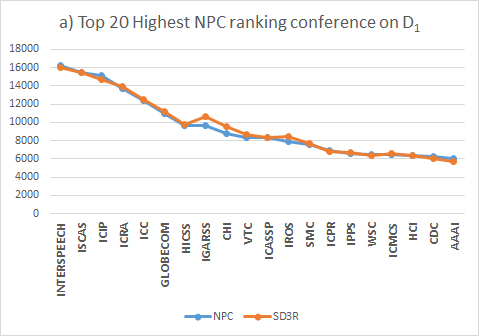
\includegraphics[width=0.45\textwidth]{D1t20cNPC}
    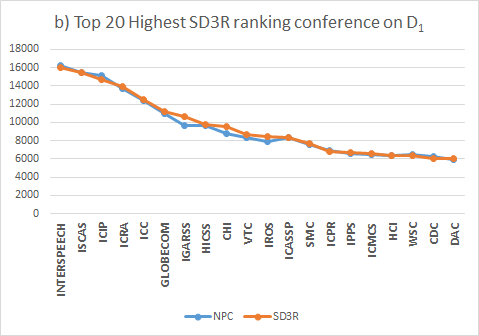
\includegraphics[width=0.45\textwidth]{D1t20cSD3R}
    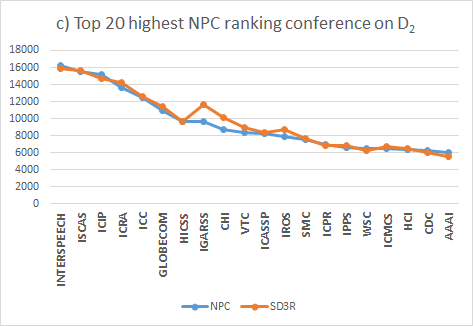
\includegraphics[width=0.45\textwidth]{D2t20cNPC}
    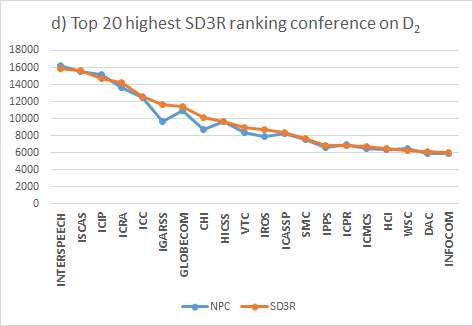
\includegraphics[width=0.45\textwidth]{D2t20cSD3R}
\end{figure}

\begin{remark}
The rank score of conferences in SD3R and NPC model are almost the same, but $\Delta^{NPC,SD3R}$ reflects how hot the conferences are.
\end{remark}

Figure \ref{Fig:Top20Conference} shows that all most of top 20 conference ranking values are the same for both methods and in both dataset $D_1, D_2$. There is a slightly different values of top 20 conferences between $D_1$ and $D_2$, since $D_2$ contains only conferences having more than 300 publications. 
Figure \ref{Fig:DeltaRho} shows that the average of $\%\Delta^{SD3R, NPC}_c$ of conferences is small, less than $0.1$ for both $D_1$ and $D_2$. It also emphasizes that SD3R and NPC methods give very similar results when ranking conferences.
The Spearman correlation coefficient of ranking conferences $\rho_c(SD3R,NPC)$ near by 1.0 indicates that the conference ranking scores of both methods are perfect monotone.
%
\begin{figure} %this figure will be at the right
	\caption{Top 5 most different ranking scores of conferences by SD3R vs. NPC over $D_1$ and $D_2$, $\alpha_2=0.45$}
	\label{Fig:Top5Inc}
    \centering
    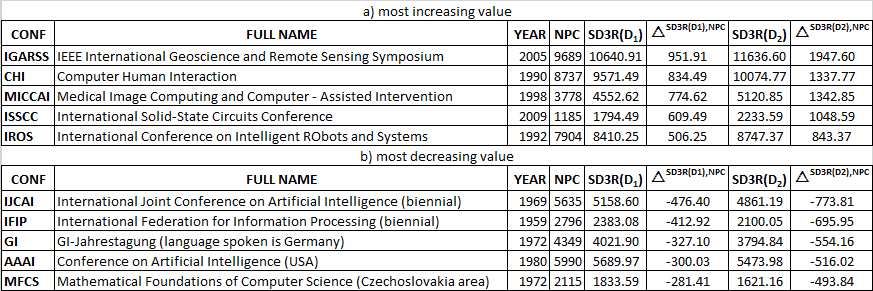
\includegraphics[width=0.9\textwidth]{Top5cInc}
\end{figure}
%
%
\begin{figure} 
	\caption{The different ranking scores values by SD3R vs. NPC, $\alpha_2=0.45$}
	\label{Fig:DeltaRho}
    \centering
    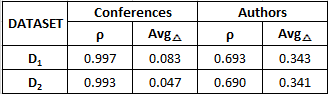
\includegraphics[width=0.5\textwidth]{delta_rho}
\end{figure}
%

Figure \ref{Fig:Top5Inc}-a shows   \textit{increasing} conferences are young, annual events and get hot topics, such as remote sensing (IGARSS), computer human interaction (CHI), medical image computing (MICCAI), solid-state circuits (ISSCC), intelligent robot (IROS). On the other hand, Figure \ref{Fig:Top5Inc}-b shows the top five \textit{decreasing} conferences are held for over a long time or biennial events, in local community (GI, MFCS) or long exploited topics such as artificial intelligence (IJCAI, AAAI), image processing(IFIP).
\begin{remark}
SD3R ranks authors differently and reflects the contribution of the author betters than NPC.
$\Delta^{NPC,SD3R}$ helps us  detecting the key authors.
\end{remark}
The $Avg_{\Delta}(SD3R,NPC)$ of authors in $D_1$ and $D_2$ are around $34\%$ (See Figure \ref{Fig:DeltaRho}). It indicates the rank scores of authors in \textit{SD3R} and \textit{NPC} models are significantly different. Figure \ref{Fig:Top20AuthorIncDec} shows that SD3R is quite different from NPC in the case of the top 20 most different ranking scores of authors.

We realize that most authors in the top \textit{decreasing} ranking values have a large number of publications (See more detail in Figure \ref{Fig:Top5AuthorDec}, about five authors in Figure \ref{Fig:Top20AuthorIncDec}-b, Figure \ref{Fig:Top20AuthorIncDec}-d). These authors have a large number of co-authors publications and belonging many different conferences.  

\begin{figure} 
	\caption{Top 20 most different ranking scores of authors by SD3R vs. NPC, $\alpha_2=0.45$}
	\label{Fig:Top20AuthorIncDec}
    \centering
    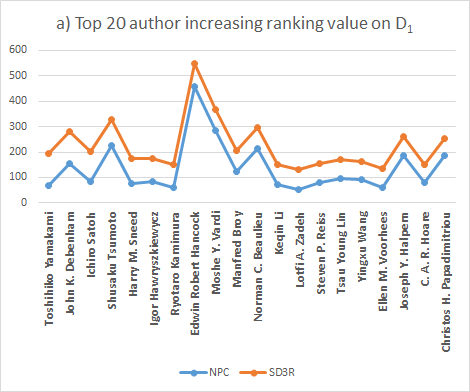
\includegraphics[width=0.45\textwidth]{D1t20aINC}
    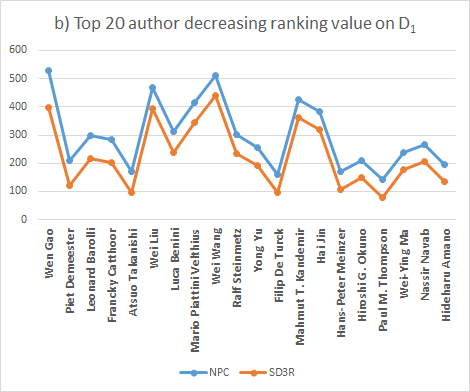
\includegraphics[width=0.45\textwidth]{D1t20aDEC}
    \includegraphics[width=0.45\textwidth]{D2t20aINC}
    \includegraphics[width=0.45\textwidth]{D2t20aDEC}
\end{figure}
%
%
\begin{figure} %this figure will be at the right
	\caption{Top 5 most decreasing ranking scores of authors having biggest NPC}
	\label{Fig:Top5AuthorDec}
    \centering
    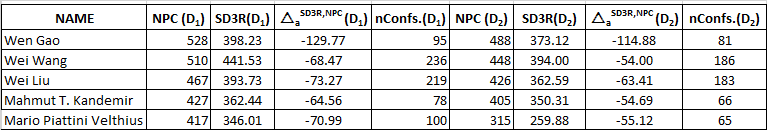
\includegraphics[width=0.9\textwidth]{T5adec}
\end{figure}
%
%
\begin{figure} %this figure will be at the right
	\caption{Top 5 most increasing ranking scores of authors having smallest NPC}
	\label{Fig:Top5AuthorInc}
    \centering
    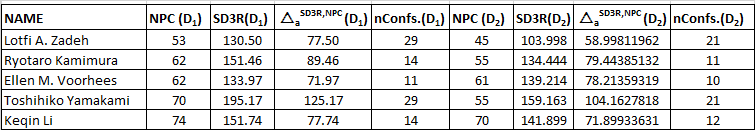
\includegraphics[width=0.9\textwidth]{T5ainc}
\end{figure}
%
From Figure \ref{Fig:Top20AuthorIncDec}-a and Figure \ref{Fig:Top20AuthorIncDec}-c, we observe that most of top \textit{increasing} authors do not have a big number of publications. Most of their papers have only one author and are published in some specialized conferences. Additionally, in Figure \ref{Fig:Top5AuthorInc}, we find out they are really key-person in their research topics in real life, such as:
\begin{itemize} 
\item \textit{Emeritus Professor  Lotfi A. Zadeh} %\footnote{http://en.wikipedia.org/wiki/Lotfi$\_$A.$\_$Zadeh} 
at the University of California, Berkeley invented the theory of fuzzy sets.
\item \textit{Professor Ryotaro Kamimura} at Tokai University %\footnote{http://65.54.113.26/Author/3332281/ryotaro-kamimura}
specializes on Machine Learning and Pattern Recognition; 
\item \textit{Ellen M. Voorhees} at NIST%\footnote{http://www.linkedin.com/pub/ellen-voorhees/6/115/3b8}
, is very famous from international workshops series: the Text REtrieval Conference (TREC), TREC Video (TRECVid), and the Text Analysis Conference (TAC).
\item \textit{Senior Specialist Toshihiko Yamakami}%\footnote{http://www.linkedin.com/pub/toshihiko-yamakami/18/649/564}
, at ACCESS, Japan Advanced Institute of Science and Technology, is professional on Mobile Social Application; 
\item \textit{Professor Keqin Li}
%\footnote{http://www.cs.newpaltz.edu/$\sim$lik/} 
 is from State University of New York at New Paltz, notable for parallel and distributed computing.
\end{itemize}

Also from Figure \ref{Fig:Top20AuthorIncDec}-a and Figure \ref{Fig:Top20AuthorIncDec}-c, there are some special cases in increasing ranking list, in which authors have big NPC ranking scores. We suppose that it is because almost of their paper are published in high ranking score conferences. Some example authors are as following: 
\begin{itemize}
\item \textit{Edwin Hancock} is a very well known scientist on computer vision;
% \footnote{http://scholar.google.com/citations?user=EjDU2ncAAAAJ};
\item \textit{Norman C. Beaulieu}, an Canadian engineer and professor in the ECE department of the University of Alberta is very famous in broadband digital and communications systems;
\item \textit{Professor Irith Pomeranz}, affiliated at School of Electrical and Computer Engineering, Purdue University %\footnote{https://engineering.purdue.edu/$\sim$pomeranz/}
is noble for Computer Engineering
VLSI and Circuit Design.
\end{itemize}
\subsubsection{SC4R, H-index, NCC, NPC}
\begin{remark}
In the case of citations are considered, SC4R is more fine-grained than NPC and NCC on the conference ranking problem. Moreover, the citations is the main factor making the rank score meaningful.
\end{remark}

Because of the naive feature of counting, both NPC and NCC methods treat the citations or publications separately. There may be too many authors having the same NPC or NCC value. With SC4R, all citations and publications are ranked together, thus the SC4R rank scores seem to be more meaningful. 
The different ranking measurement figures are shown in Figure \ref{Fig:DiffRank}.
The Kendall' tau coefficients points out that ranking by SC4R is more concordant with NCC than NPC method, and each pair of them is not quite the same concordant. It confirms again the fact that citation is the main factor for ranking scientific publications.

\begin{figure}
	\caption{Different ranking measurement of SC4R with $\alpha_1=0.3$ vs. NPC, NCC, H-index on $D_c$}
	\label{Fig:DiffRank}
    \centering
    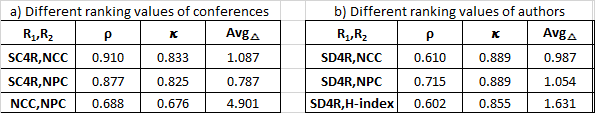
\includegraphics[width=0.95\textwidth]{DiffRank}
\end{figure}
%
%
\begin{remark}
SC4R seems to be in the middle of the popularity and the prestige ranking of conferences.
\end{remark}
Figure \ref{Fig:Top20ConfDc} shows the trend of SC4R lines in top ranking value from three methods. In each graph, the SC4R line always fluctuate between NPC (popularity) line and NCC (prestige) line, nearly coincides to the average of them. 


Figure \ref{Fig:Top10ConfDc} shows top 10 rank position by SC4R methods compare to compliled lists of MS RANK \cite{microsoft} and CORE RANK \footnote{http://www.core.edu.au/coreportal. Accessed on May -25, 2014.}.  
Let us see three interesting cases:
\begin{itemize} 
\item \textit{VLDB vs. HICSS.} The number of articles published in HICSS is fivefold of VLDB's but HICSS$'$s cited papers are just a fourth of VLDB. In our SC4R method, VLDB stands before HICSS. Their SC4R ranking values are 8403.14 and 7037.91 respectively, totally not far different.

\item \textit{PODS and ISWC}. We can easily point out two prestige database conferences, PODS and ISWC, which has not in top 10 in popularity, being 18 and 16 respectively.

\item \textit{DEXA and ICEIS}. We can see two low -ranked conferences by MS RANK and CORE experts assessment are listed in top 10 of SC4R conference rank, DEXA and ICEIS. This can be explained by the experimental dataset $D_c$ contains many papers as well as citations of these two conferences. DEXA has 3982 papers and that number of ICEIS is 2993.
\end{itemize}

It is impressive that most of the top 10 of SC4R conference ranking list are the most noble in database field following the assessment of CORE experts and Microsoft Academic Search system.

\begin{figure} 
	\caption{Top highest ranking value of conferences by NPC, NCC and SC4R on $D_c$ with $\alpha_1=0.3$}
	\label{Fig:Top20ConfDc}
    \centering
    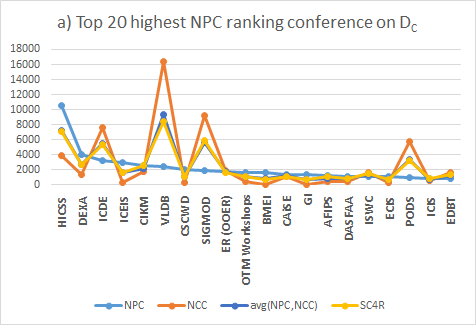
\includegraphics[width=0.45\textwidth]{Dct20NPCc}
    \includegraphics[width=0.45\textwidth]{DCt20NCCc}
    \includegraphics[width=0.90\textwidth]{DCt40SC4Rc}   
\end{figure}
%
\begin{figure}
	\caption{Top 10 SC4R rank position of conferences on $D_c$ with $\alpha_1=0.3$}
	\label{Fig:Top10ConfDc}
    \centering
    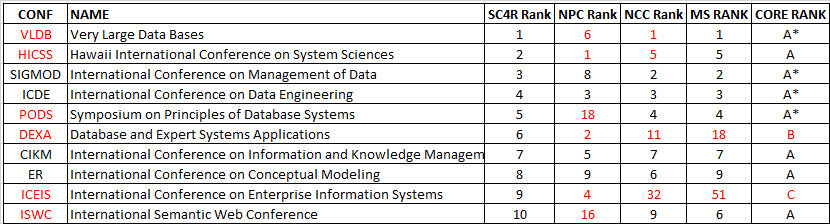
\includegraphics[width=0.95\textwidth]{Top10Conf}
\end{figure}
%
\begin{remark}
SC4R seems to reflect the contribution of the author better than others from combining prestige and popularity criteria. 
\end{remark}

Figure \ref{Fig:Top20AuthorDc}-a shows the top 20 highest NPC ranking author value.  H-index line is the lowest line and separated with other lines. It can be explained that  many authors have published a big number of papers which get a few citations. We remind that H-index is proposed for the combination of popularity and prestige value of an author. Let us see other three graphs of Figure 10, which show the ranking values by NCC (focus on prestige), H-index (combining popularity and prestige) and SC4R. We found that H-index nearly coincides with NPC line. We suppose that H-index extremely falls into quantity pole in these case. Meanwhile, the NCC line, standing for the prestige of author via high citation, is always the highest line in Fig.~\ref{Fig:Top20AuthorDc}-b, Fig.~\ref{Fig:Top20AuthorDc}-c, Fig.~\ref{Fig:Top20AuthorDc}-d. SC4R does not fall extremely into popularity (NPC, H-index) or prestige (NCC) poles. Thus SC4R is the good method to reflecting the contribution of author in which combines prestige and popularity criteria. 

Let's look detail for some special authors in Fig.~\ref{Fig:Top20AuthorDetail}. 

\begin{itemize}
\item \textit{Professor Jennifer Widom and Alon Halevy}. They fall in the case of high citation, high H-index, high publications but lower SC4R. 
The citation number of Professor Jennifer Widom
%\footnote{http://infolab.stanford.edu/~widom/}
is nearly double than that of Michael Stonebraker, a pioneer of data base research and technology %\footnote{https://www.csail.mit.edu/user/1547}
. She also has H-index higher than Michael Stonebraker 
%\footnote{https://www.csail.mit.edu/user/1547} 
but her number of publications is lower than his one. We can see her SD4R value is a bit lower than Michael Stonebraker's SD4R value. We assume the result is because many publications citing to her papers do not get high score in SC4R ranking, namely not good quality.
\item \textit{Jim Gray, Antonin Guttman and Umeshwar Dayal}. They fall in the opposite situation in which all authors have low NPC, NCC and H-index value, but high SD3R score. This situation can be explained by their publications are cited by almost prestige people and high quality publications and are published in noble conferences.
\end{itemize}

We review the top 20 highest SC4R value people and find out that they all are very famous in database field with many valuable scientific works.

\begin{figure} %this figure will be at the right
	\caption{Top 20 ranking value of author by NPC, NCC, H-index* and SC4R on $D_c$ with $\alpha_1=0.3$}
	\label{Fig:Top20AuthorDc}
    \centering
    \includegraphics[width=0.45\textwidth]{DCt20NPCa}
    \includegraphics[width=0.45\textwidth]{DCt20NCCa}
    \includegraphics[width=0.45\textwidth]{DCt20Hindexa}
    \includegraphics[width=0.45\textwidth]{DCt20SC4Ra}
\end{figure}

\begin{figure} %this figure will be at the right
	\caption{Top 20 SC4R ranking value on $D_c$ with $\alpha_1=0.3$}
	\label{Fig:Top20AuthorDetail}
    \centering
    \includegraphics[width=0.95\textwidth]{DCt20SC4Ra-f}
\end{figure}
%

\section{Related work}\label{Sect:Related}
\textit{Our prior work}. Our work is the extend version of the prior work \cite{Vu14}. In this version, we has extend the experiments and represent everything more in detail. Concretely, we do the experiments for the case the citations are considered. We also compare our ranking with the H-index, which is the most famous ranking scores for authors recently. Moreover, we improve the results by giving more discussions.

\textit{Web-pages ranking}. The ranking problem occurs and develop quickly with the era of the Internet and big data. One of the most famous ranking problem is ranking web-pages. A brief overview of this problem can be found at Dilip Kumar Sharma et al. \cite{RankOverview}. The recent survey on web-pages ranking algorithms was conducted by Mercy Paul Selvan et. al. \cite{SurveyWebRank}. They categorized these ranking algorithms into three groups: i)Link analysis algorithms, ii) Personalized web search ranking algorithms and iii) Page Segmentation algorithms. 
The first group is highlight by two notable classical algorithms, naming PageRank \cite{pagerank98} utilized by Google search engine and Hyperlink-Induced Topic  Search (HITS) \cite{HITS} developed by Jon Kleinberg.
Since the hyperlink structure among the web-pages are easily represented as a web graph,
the PageRank of each web-page can be measured (see Sect.~\ref{Sect:PageRank} for more detail). HITS was a precursor to PageRank. The idea behind HITS algorithm classify the webs into two classes: (i) hubs, served as large directories point to (ii) authoritative pages. A good hub represented a page that pointed to many other pages, and a good authority represented a page that was linked by many different hubs. The model can be rewritten into 2-linear ranking model.
The advantages and disadvantages of link analysis algorithms are also discussed in works of Dilip Kumar Sharma et al. \cite{RankOverview} and Mercy Paul Selvan et. al. \cite{SurveyWebRank}. 

\textit{Link-based object ranking}. The basic problems of link-based object ranking can be found at the survey on link mining of Getoor and Christopher P. Diehl \cite{LinkMining}. Zaiqing Nie et. al. proposed Poprank model \cite{poprank} to rank the popularity of objects based on their web popularity and the object relationship graph. It extends from PageRank and uses the Popularity Propagation Factor to express the relationship between classes of objects. The model is based on the markov chain model which can be applied in the N-linear mutual ranking systems.
Yizhou Sun et. al. proposed NetClus algorithm \cite{NetClus} that utilizes links between objects of multi-typed to rank cluster of multi-typed heterogeneous networks. This work is the successor of their previous work, RankClus, which can rank and cluster one-typed objects mutualy \cite{RankClus}. Their model is the same idea with ours when limiting only within a star network schema and giving rank distribution for each type of objects. But our approach is different from theirs. NetClus's objects in the center class (target type) only relates to those belong to other classes (attribute types). So it can not be applied to compute on the citation network. Other complex ranking systems have been already explored using a different formalism for ranking or classification in heterogeneous networks. For example, the quantium ranking \cite{complexrank} is based on quantium navigation. Their formula is come from the quantium theory and quite different to ours.

\textit{Bibliometric ranking}. 
Many methods of assessing the intellectual impact, reputation and influence of scientists, journals, conferences have been proposed over years. In a very recent scientometric study \cite{EvaluatingJournal}, Paul Benjamin Lowry et. al. compare expert assessments to bibliometric measures for determining a tiered structure of information systems (IS) journals. They categorize the assessing journal quality methods into three methodology paths: (i) bibliometric-based, (ii) expert-based and  (iii) non-validated approach.
One of their noticeable conclusion is that bibliometrics can be a complete, less expensive and more efficient substitute for expert assessment. For bibliometric approaching, many detailed definitions of citation metrics can also be found in this paper, such as the most used ISI Impact Factor, h-index and it variants like g-index, e-index\ldots Another study of bibliometric graph-based algorithms focus on ranking researchers was conducted by Xiaorui Jiang et. al \cite{Graphbased}. They compare sophisticated citation analysis algorithms like PageRank, SARA, CoRank, FutureRank, P-Rank, BiRank with some simpler methods like citation count and sum of paper ranks, similar to the way we evaluate the experiment results. Further information about bibliometrics and web-based citation analysis can be seen on \cite{Cronin-JIS-01}.  

%%%%%%%%%%%%%%%%%%%%%%%%%%%%%%%%%%%%%%%%%%%%%%%%%%%%%%%%%%%%%%%%%%
\section{Conclusion and future works}\label{Sect:Conclusion}
We have introduced and studied N-linear ranking systems. The mutual relationships between ranking objects are described by a system of linear equations. A N-linear mutual ranking system is a N-star ranking systems if it has a core class which affects and reflects all other classes in the system. The rank scores of the N-star ranking system are unique and computed by a loop of computing the linear function. We have pointed out that PageRank is a 2-star ranking. It has two classes:  the web-pages (a core class) and links.

We have introduced and studied a general and a simple 4-star ranking models for ranking authors, publications, conferences. A general model is a generic one. In a simple model, we consider each publication, author, conference, citation is equally. We have conducted the experiments for the models in two contexts with/without citations. The experimental results are based on the DBLP dataset. We have compared the difference of the values and the concordance between the proposed ranking systems (SD3R and SC4R) and naive, classical ranking systems (NPC, NCC, H-index). We have found that: 
\begin{itemize}
\item In the case citations are not considered, the rank score of conferences in SD3R and NPC model are almost the same, but $\Delta^{NPC,SD3R}$ reflects how hot the conferences are. SD3R ranks authors differently and reflects the contribution of the author betters than NPC.
\item The citations are the main factors for measuring the prestige of a publications, conferences and authors. SC4R seems to reflect the rank of the author, the conference better than others from combining prestige and popularity criteria.
\end{itemize}

As future work, we are planning to $i$) Develop the current system to retrieve big data including publications and  citations  $ii$) Study how to combine the proposed ranking system with class keywords, which are tagged in the publications $iii$) investigate the time series in N-star ranking and the trend prediction problem, and $iv$) Apply N-star ranking systems in various ranking problems, e.g., business ranking, event ranking, and so on.

\vspace{-3ex}
\begin{thebibliography}{99}
\setlength{\parskip}{-3pt}\vspace{-2ex}

\bibitem{HIndex06}
\textbf{A. Sidiropoulos, D. Katsaros, Y. Manolopoulos.}
Generalized Hirsch h-index for disclosing latent facts in citation networks.
\textit{Scientometrics,} \textbf{Vol. 72 (2)}, (2006), 253--280.

\bibitem{Cronin-JIS-01}
\textbf{Blaise Cronin.}
Bibliometrics and beyond: some thoughts on web-based citation analysis.
\textit{Journal of Information Science},
\textbf{Vol. 27 (1)}, (2001), 1--7.

\bibitem{complexrank}
\textbf{Eduardo Sánchez-Burillo, Jordi Duch, Jesús Gómez-Gardenes, David Zueco},
Quantum Navigation and Ranking in Complex Networks,
\textit{Scientific reports 2}, (2012).

\bibitem{LinkMining}
\textbf{Getoor, Lise, and Christopher P. Diehl},
Link mining: a survey,
\textit{ACM SIGKDD Explorations}
\textbf{Newsletter 7 (2)}, (2005), 3-12.

\bibitem{HIndex}
\textbf{J. E. Hirsch},
An index to quantify an individual's scientific research output,
\textit{Proceedings of the National Academy of Sciences of the United States of America}, \textbf{102(46)}, (2005), 16569–-16572.


\bibitem{Keener1993}
\textbf{J. Keener.},
The Perron-Frobenius theorem and the ranking of football teams,
\textit{SIAM Review} \textbf{ 35(1)}, (1993), 80--93.

\bibitem{HITS}
\textbf{Jon Kleinberg},
Authoritative Sources in a Hyperlinked Environment,
\textit{Journal of the ACM}, \textbf{Vol. 46 (5)}, (1999), 604-632.


\bibitem{Kien09}
\textbf{L. T. Kien, L. T. Hieu, T. L. Hung, L. A. Vu.},
MpageRank: The Stability of Web Graph.
\textit{Vietnam Journal of Mathematics}, \textbf{Vol. 37}, (2009), 475--489.

\bibitem{Kendall1938}
\textbf{M.G. Kendall.},
A new measure of rank correlation,
\textit{Biometrika}, (1938), 81--93.

\bibitem{SurveyWebRank}
\textbf{Mercy Paul Selvan, A .Chandra Sekar, A.Priya Dharshin},
Survey on Web Page Ranking Algorithms,
\textit{International Journal of Computer Applications},
\textbf{Vol. 41 (19)}, (2012), 1--7.
%

\bibitem{MichaelLey09}
\textbf{Michael Ley.}
DBLP - Some Lessons Learned.
\textit{PVLDB} 2 (2), (2009), 1493--1500.


\bibitem{MichaelLey06}
\textbf{Michael Ley, Patrick Reuther.}
Maintaining an Online Bibliographical Database: The Problem of Data Quality.
\textit{EGC 2006}, 5--10.

\bibitem{microsoft}
\textbf{Microsoft  Corporation.}
Microsoft Academic Search.
\textit{http://academic.research.microsoft.com/} (June -26 -2013).

\bibitem{EvaluatingJournal}
\textbf{Paul Benjamin Lowry, Gregory D. Moody, James Gaskin, Dennis F. Galletta, Sean L. Humpherys, Jordan B. Barlow, and David W. Wilson},
Evaluating Journal Quality and the Association for Information Systems Senior Scholars' Journal Basket Via Bibliometric Measures: Do Expert Journal Assessments Add Value?.
\textit{The MIS Quarterly},
\textbf{Vol. 37 (4)}, (2013), 993--1012. 

%
\bibitem{Nelsen2006}
\textbf{R.B. Nelsen.}
\textit{An Introduction to Copulas, 2nd ed.}.
Springer Series in Statistics, Springer, (2006), New York.


\bibitem{pagerank98}
\textbf{S. Brin and L. Page.}
The anatomy of a large-scale hypertextual web search engine.
\textit{Proceedings of the 7th International World Wide Web Conference}, (1998), 107--117.

\bibitem{spearman}
\textbf{Charles Spearman},
"General Intelligence," Objectively Determined and Measured,
\textit{The American Journal of Psychology}
\textbf{ 15 (2)}, (1904), 201--292.


\bibitem{RankOverview}
\textbf{Sharma, Dilip Kumar and Sharma A. K},
A comparative analysis of web page ranking algorithms,
\textit{International Journal on Computer Science and Engineering}, (2010), 2670--2676.

\bibitem{Vu14}
\textbf{Vu L. A., Hai V. H., Kien L. T., Hieu L. T., Jason J. Jung},
A General Model for Mutual Ranking Systems,
\textit{Intelligent Information and Database Systems, Lecture Notes in Computer Science}, 
\textbf{Vol. 8397}, (2014), 211--220.

\bibitem{Graphbased}
\textbf{Xiaorui Jiang, Xiaoping Sun, and Hai Zhuge}, Graph-based algorithms for ranking researchers: not all swans are white!,
\textit{Scientometrics},
\textbf{Vol. 96 (3)}, (2013), 743--759.

\bibitem{NetClus}
\textbf{Yizhou Sun, Yintao Yu, Jiawei Han},
Ranking-based clustering of heterogeneous information networks with star network schema,
\textit{Proceedings of the 15th ACM SIGKDD international conference on Knowledge discovery and data mining},
(2009), 797-806.

\bibitem{RankClus}
\textbf{Yizhou Sun,Jiawei Han, Peixiang Zhao, Zhijun Yin, Hong Cheng, Tianyi Wu},
Rankclus: integrating clustering with ranking for heterogeneous information network analysis,
\textit{Proceedings of the 12th International Conference on Extending Database Technology: Advances in Database Technology, ACM}, (2009), 565--576. 

\bibitem{poprank}
\textbf{Zaiqing Nie, Yuanzhi Zhang, Ji-Rong Wen, and Wei-Ying Ma},
Object-level ranking: bringing order to web objects,
\textit{Proceedings of the 14th international conference on World Wide Web, ACM}, (2005), 567--574.


\end{thebibliography}
\vspace{2cm}

\noindent\textbf{Vu Le Anh}\\
Nguyen Tat Thanh University\\
Ho Chi Minh City\\
Vietnam\\
{\tt e-mail lavu@ntt.edu.vn}\\

\noindent\textbf{Vo Hoang Hai}\\
Information Technology College\\
Ho Chi Minh city\\
Vietnam\\
{\tt e-mail vohoanghai2@gmail.com}\\

\noindent\textbf{Hieu Le Trung}\\
Duy Tan University\\
Da Nang\\
Vietnam\\
{\tt e-mail hieukien82@gmail.com}\\

\noindent\textbf{Kien Le Trung}\\
Hue University of Science\\
Thua Thien Hue\\
Vietnam\\
{\tt e-mail hieukien@hotmail.com}\\

\noindent\textbf{Jason J. Jung}\\
Chung-Ang University\\
Seoul\\
Korea\\
{\tt e-mail j2jung@gmail.com }

\end{document}
